\subsection{Scénario Cockburn}
\textbf{Cas d'utilisation:} Payer le passage

\textbf{Acteur primaire:} Le conducteur

\textbf{Acteur support:} Le poste de surveillance et opérateur humain (si le borne est manuelle)

\textbf{Pré-condition: }  la borne est opérationnelle

\textbf{Scenario primaire: } \\ 
    \textbf{1.} Le conducteur paye par carte bleu %(\ref{subsec:paierBleu})
    \\ 

\textbf{Variantes:}\\
    \textbf{1a.} Le conduteur paye en liquide %(\ref{subsec:paieLiquide})
    \\
    \textbf{1b.} Le conducteur paye par carte abonnement %(\ref{subsec:paierAbonement})
    \\
     \textbf{1c.} Le conducteur paye par telépéage.
     \\
    \textbf{1d.} Le paiement a échoué. Retourne à l’état 1. \\ %he clicks in the botton who calls the technicien 

\subsection{Décomposition de cas d'utilisation (Généralisation):} 
\begin{figure}[h]
    \centering
    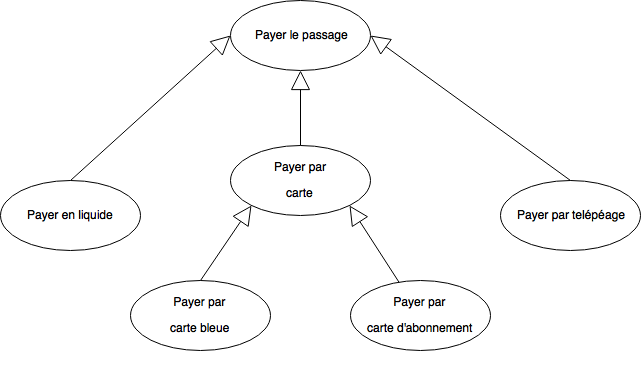
\includegraphics[scale=0.5]{02_Desenvolvimento/TD2/images/PayeGeneralisation.png}
    \caption{Généralisation de cas d'utilisation: Payer le passage}
\end{figure}

\subsection{Diagramme d'activité}
\begin{figure}[h]
    \centering
    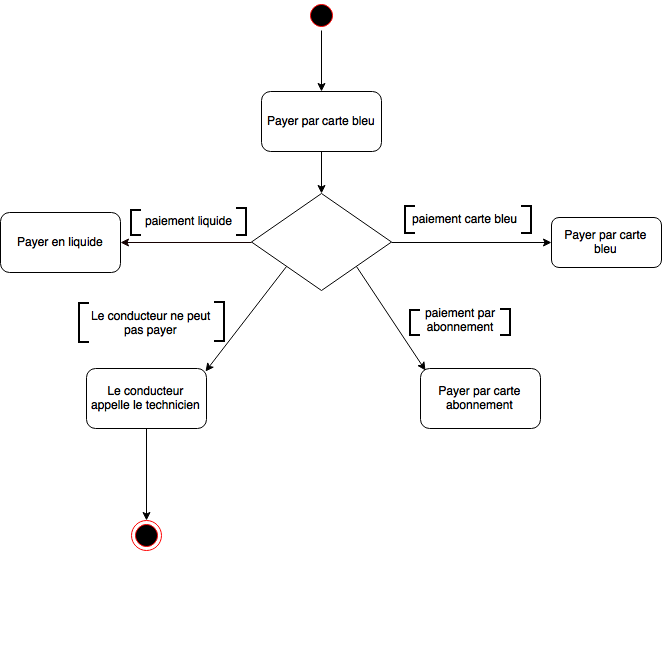
\includegraphics[scale=0.6]{02_Desenvolvimento/TD2/images/DAPayePassage.png}
    \caption{Diagramme d'activité: Payer le passage}
\end{figure}
\newpage
\subsection{Collaboration}
\begin{figure}[h]
    \centering
    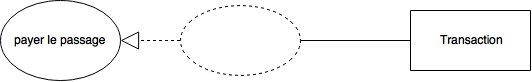
\includegraphics[scale=0.6]{02_Desenvolvimento/TD2/images/ColaPayer.png}
    \caption{Diagramme d'activité: Payer le passage}
\end{figure}
